\documentclass[a4paper, 11pt]{article}

\usepackage[left=1.5cm, right=1.5cm, top=2cm, bottom=2cm]{geometry}

\usepackage[utf8]{inputenc} 
\usepackage[T1]{fontenc}      
\usepackage[french,english]{babel}  
\usepackage{lmodern}

\usepackage{amsmath, mathtools}
\usepackage{amssymb}
\usepackage{amsthm}
\usepackage{empheq}

\usepackage{graphicx,wrapfig}
\usepackage{subfig}

\usepackage{listings}
\usepackage{color} %red, green, blue, yellow, cyan, magenta, black, white
\definecolor{mygreen}{RGB}{28,172,0} % color values Red, Green, Blue
\definecolor{mylilas}{RGB}{170,55,241}

\graphicspath{{../figures/}}
\usepackage{caption}

\begin{document}
\title{Rendu DM3 Optimisation Convexe} 
\author{Yoann Pradat}
\maketitle

\textbf{1}. Let's derive the dual of the LASSO problem in the variable $w \in \mathbf{R}^d$. 

\begin{equation}
  \min_{w \in \mathbf{R}^d} \frac{1}{2} \| Xw-y \|_2^2 + \lambda \| w \|_1
\end{equation}

where $\lambda \in \mathbf{R}$, $X \in \mathbf{R}^{n\times d}$ and $y \in \mathbf{R}^n$ are fixed. The LASSO problem is
equivalent to the constrained problem over $(v,w) \in \mathbf{R}^{n\times d}$

\begin{align}
  \min_{(v,w) \in \mathbf{R}^{n\times d}} &\frac{1}{2} \| v \|_2^2 + \lambda \| w \|_1 \\
  \text{s.t} \quad &  Xw-y = v \nonumber
\end{align}

Let $f_0: (v,w) \mapsto f_1(v) + f_2(w)$ be the objective function with $f_1: v \mapsto \frac{1}{2} \|v\|_2^2$ and $f_2:
w \mapsto \lambda \|w\|_1$. Let's compute the conjugage of $f_0$, it will be useful in the formulation of the dual problem. First
notice that $f_1$ and $f_2$ are convex and that $f_0$ is a function of two variables but that these variables are
separated. Consequently, the conjugate of $f_0$ is the sum of the conjugates of $f_1$ and $f_2$ i.e $f_0^*(s,t) =
f_1^*(t) + f_2^*(s)$. \\

The conjugate of $f_1$ is $f_1^*(t)=\frac{1}{2} \| t\|_{*,2}^2$ where $ \| t\|_{*,2} = \sup\{t^Tv | \|v\|_2 \leq 1 \}$. Indeed
let $t \in \mathbf{R}^n$. Then 

\begin{align*}
  \forall v  &\in \mathbf{R}^n \quad  t^Tv \leq \|t\|_{*,2} \|v\|_{2} \\
  &\implies t^Tv - \frac{1}{2}\|v\|_2^2 \leq \|t\|_{*,2} \|v\|_{2} - \frac{1}{2}\|v\|_2^2  \\
  &\implies t^Tv - \frac{1}{2}\|v\|_2^2 \leq \frac{1}{2} \|t\|_{*,2}^2
\end{align*}

as the left-hand side on the second line is a quadratic function of $\|v\|_2$ with maximum $\frac{1}{2}\|t\|_{*,2}^2$.
Therefore, $f_1^*(t) \leq \frac{1}{2} \|t\|_{*,2}^2$. Now, let $v \in \mathbf{R}^n$ be such that $t^Tv  =  \| t\|_{*,2} 
\|v\|_2$. We can scale $v$ so that $\|v\|_2 = \| t\|_{*,2}$. Then  $t^Tv - \frac{1}{2}\|v\|_2^2 =
\frac{1}{2}\|t\|_{*,2}^2$. As a consequence $f_1^*(t) \geq \frac{1}{2} \|t\|_{*,2}^2$ and eventually $f_1^*(t) = 
\frac{1}{2} \|t\|_{*,2}^2$. \\

The conjugate of $f_2$ is

$$
f_2^*(s) = \left\{
        \begin{array}{ll}
           0 & \quad \|\lambda s \|_{*,1} \leq 1 \\
           \infty  & \quad \text{otherwise}
        \end{array}
    \right.
$$

Let $s \in \mathbf{R}^d$. If $\|\lambda s \|_{*,1} > 1$, by definition of the dual norm there exists $w \in
\mathbf{R}^d$ with $\|w\|_1 \leq 1$ and $\lambda s^Tw > 1$. Taking $z = aw$ and letting $a\to\infty$ we have 

\begin{equation*}
  \lambda s^Tz - \|z\|_1  = a(\lambda s^Tw - \|w\|_1) \to \infty
\end{equation*}

If $\|\lambda s \|_{*,1} \leq 1$, it is easy to show that $\lambda s^Tw - \|w\|_1$ is bounded above by 0 and 0 is
attained for $w=0$. \\

\clearpage

Let's now compute the dual of the problem (2). For $\nu \in \mathbf{R}^n$ we have 

\begin{align*}
  g(\nu) &= \inf_{(v,w) \in \mathbf{R}^{n\times d}} \left( f_1(v) + f_2(w) + \nu^T(Xw - y - v) \right) \\
 & = - f_1^*(\nu) - f_2^*(-X^T\nu) - \nu^Ty
\end{align*}


Given the previous calculations, $\nu$ is dual feasible if and only if $\|\lambda X^T \nu \|_{*,1} \leq 1$. The dual 
norm of the $l_2$-norm is the $l_2$-norm and the dual norm of the $l_1$-norm is the $l_{\infty}$-norm. Therefore, the
dual of problem (2) is

\begin{align}
  \max_{\nu \in \mathbf{R}^{n}} & -\frac{1}{2} \| \nu \|_2^2 - \nu^Ty \\
  \text{s.t} \quad &  \|\lambda X^T \nu \|_{\infty} \leq 1 \nonumber
\end{align}

that is to say 

\begin{align}
  \min_{v \in \mathbf{R}^{n}} &  \frac{1}{2}v^Tv + v^Ty \\
  \text{s.t} \quad & X^T v \preceq \frac{1}{\lambda} \nonumber
\end{align}

The dual problem is thus obtained as a QP problem 

\begin{align}
  \min_{v \in \mathbf{R}^{n}} &  v^TQv + v^Tp \\
  \text{s.t} \quad & A^T v \preceq b \nonumber
\end{align}

where \fbox{$Q = \frac{1}{2} I_n$, $p=y$, $A = X^T$ and $b = \frac{1}{\lambda}$}. \\

\textbf{2.} We are now going to solve the dual problem (5) using a barrier method. Given $(v_0,t_0,\mu, \epsilon)$ \\

\noindent\textbf{Barrier method} \\
\textbf{Repeat}
\begin{enumerate}
  \item Centering step. Compute $v^*(t)$ by minimizing $f(v) = \left[ t(v^TQv + v^Tp) - \sum_{i=1}^d
    \log(b_i-a_i^Tv)\right]$ with $a_i^T$ is the $i^{th}$ line of A. 
  \item Update $v := v^*(t)$
  \item Stopping criterion stop if $m/t < \epsilon$
  \item Increase $t$. $t := \mu t$.
\end{enumerate}

The centering step is going to be solved using Newton method with backtracking line search that is to say \\

\noindent\textbf{Centering step} \\
\textbf{Repeat}
\begin{enumerate}
  \item $\Delta v_{nt} := -\nabla^2f(v)^{-1}\nabla f(v)$ .
  \item $\lambda^2 = \nabla f(v)^T \nabla^2f(v)^{-1}\nabla f(v)$
  \item Quit if $\frac{\lambda^2}{2} < \epsilon$
  \item Choose step size $s$ by backtrack line search.
  \item Update $v := v + s\Delta v_{nt}$.
\end{enumerate}


For fixed $t \in \mathbf{R}_{++}$, the gradient and the hessian of $f$ are

\begin{align*}
  &\nabla f(v) = t(2Qv + p) + \sum_{i=1}^d \frac{a_i}{b_i-a_i^Tv} \\
  &\nabla^2 f(v) = 2tQ + \left[ \sum_{i=1}^d \frac{a_{ik}a_{il}}{(b_i - a_i^Tv)^2} \right]_{k,l \in [\![1,n]\!]^2}
\end{align*}

For given $\alpha \in (0,\frac{1}{2}), \beta \in (0,1)$, the backtrack search is solved by \\

\noindent\textbf{Backtrack search} 
\begin{enumerate}
  \item Start at $s=1$ 
  \item Repeat $s:= \beta s$ until $f(v + s\Delta v) < f(v) + \alpha s \nabla f(v)^T\Delta v$.
\end{enumerate}

\begin{figure}[!h]
  \centering
  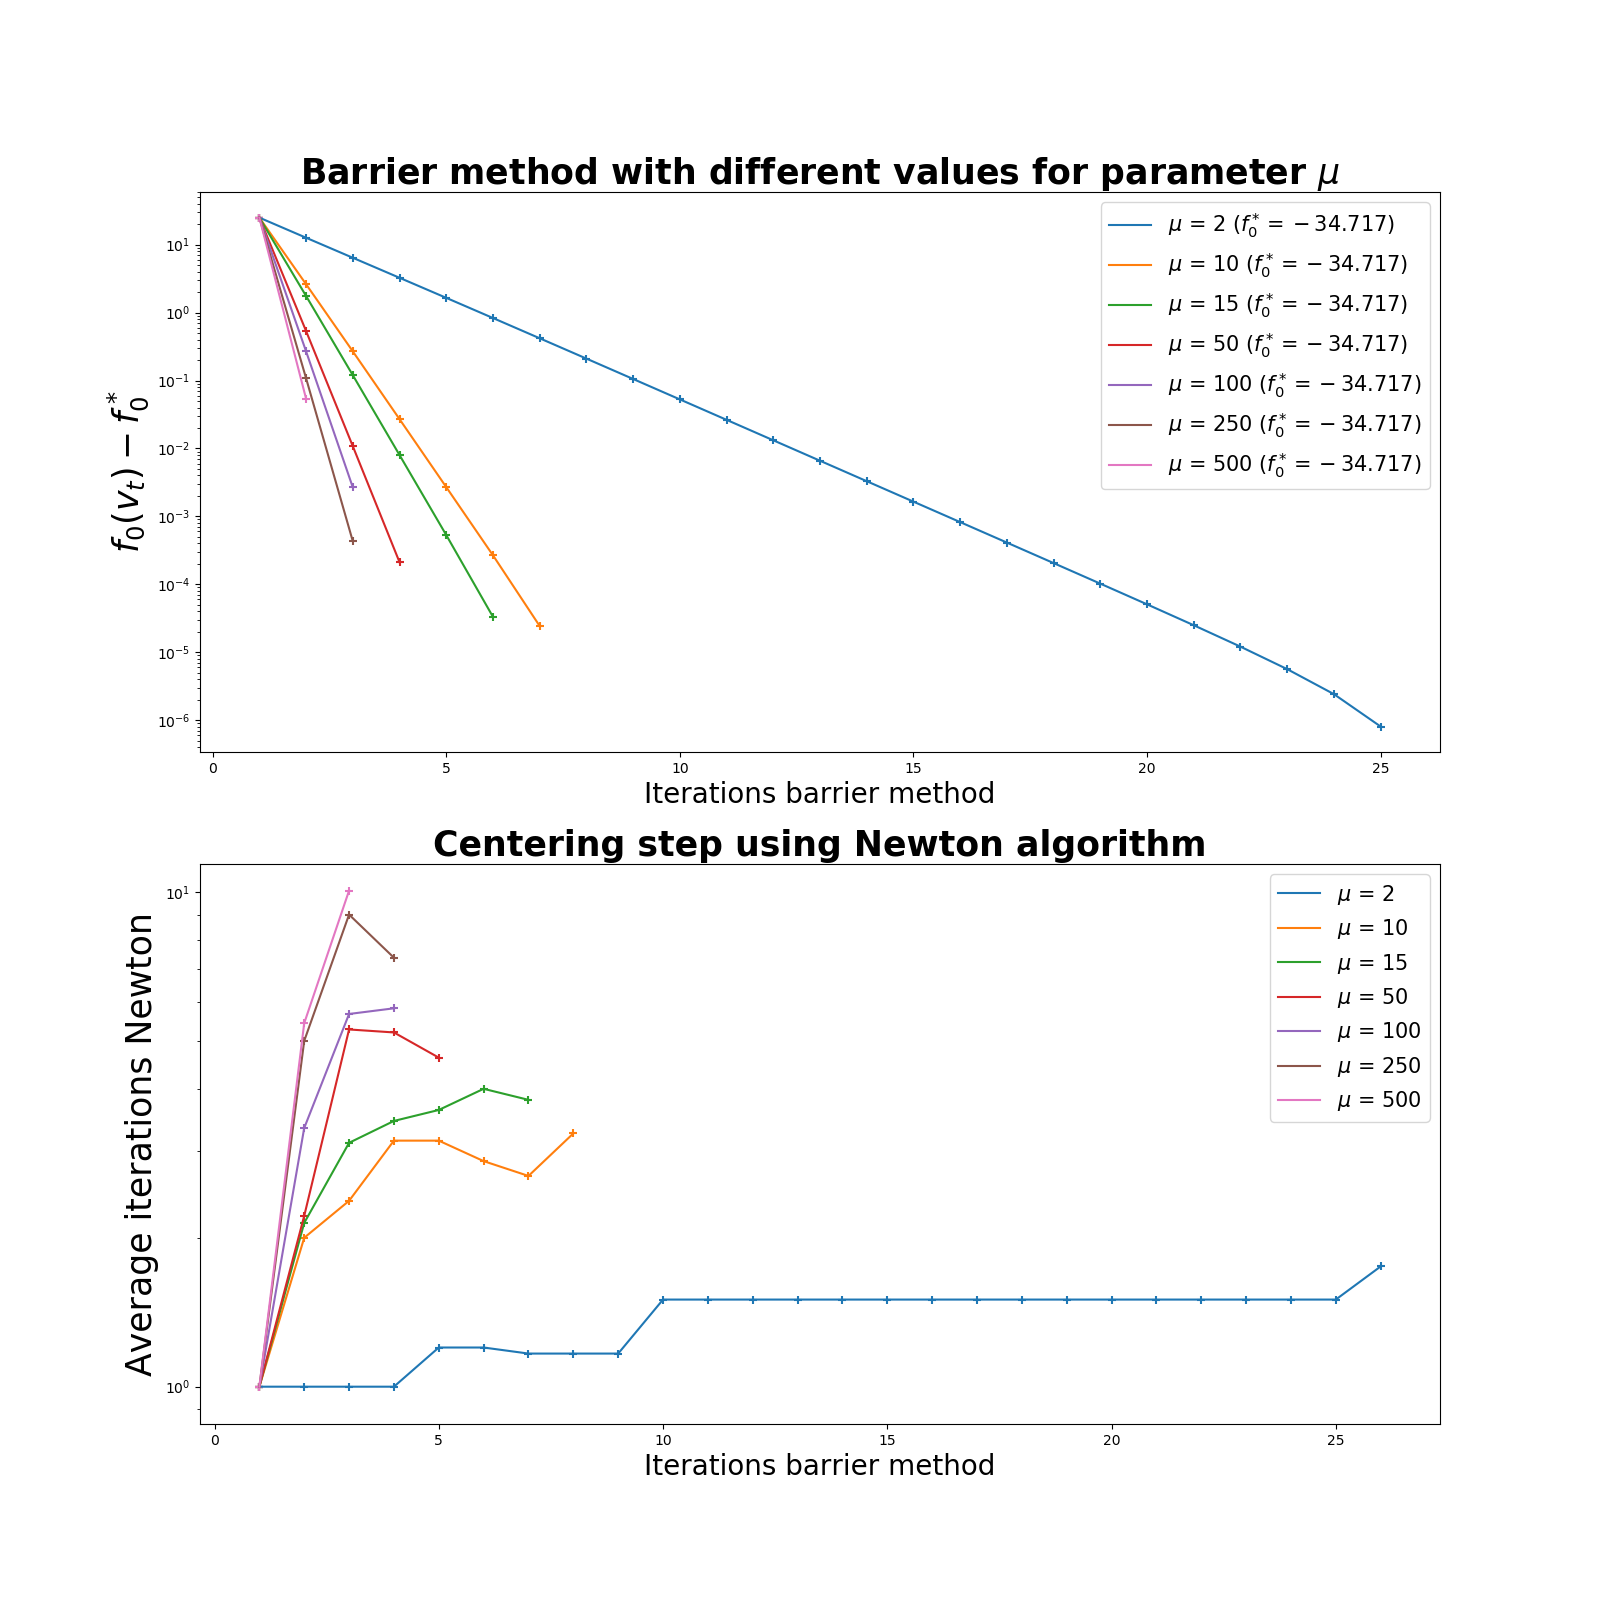
\includegraphics[width=16cm]{barr.png}
  \caption{Results barrier method on the dual of LASSO for random X and y, $\lambda=10$}
  \label{fig:barr}
\end{figure}

The constrained formulation of LASSO (2) is a convex problem for which Slater condition is satisfied. Therefore we have
strong duality. Solving the dual problem, we have a dual feasible $\nu^*$ point for (5). Then, if $(v^*, w^*)$ is
the unique solution of

\begin{equation}
  \min_{(v,w)} \left( f_1(v) + f_2(w) + (\nu^*)^T(Xw - y - v) \right) 
\end{equation}

and $(v^*, w^*)$ is primal feasible, it is primal optimal. \\

The $l_1$-norm is not differentiable on any $w \in \mathbf{R}^d$ that has at least 1 null coordinate but is
differentiable everywhere else. It is not obvious how to derive $w$ after having solved the dual problem $\ldots$

\end{document}



